% Requisitos implementados:
% - Times New Roman 12pt (cuerpo)
% - Arial negrita para títulos (14/13/12 pt)
% - Interlineado 1.5
% - Márgenes: superior/inferior/derecho 2.5 cm, izquierdo 3 cm
% - Texto justificado
% - Encabezado (derecha): nombre de asignatura y práctica
% - Pie centrado: Página X de Y

\documentclass[a4paper,12pt]{article}
\usepackage{fontspec}
\setmainfont{Times New Roman}
\newfontfamily\headingfont{Arial}
\setmonofont{Courier New}

\usepackage[a4paper,left=3cm,right=2.5cm,top=2.5cm,bottom=2.5cm]{geometry}
\usepackage{setspace}
\onehalfspacing

\usepackage{titlesec}
\titleformat{\section}{\headingfont\bfseries\fontsize{14}{16}\selectfont}{\thesection}{1em}{}
\titleformat{\subsection}{\headingfont\bfseries\fontsize{13}{15}\selectfont}{\thesubsection}{1em}{}
\titleformat{\subsubsection}{\headingfont\bfseries\fontsize{12}{14}\selectfont}{\thesubsubsection}{1em}{}

\usepackage{microtype}
\usepackage{lastpage}
\usepackage{fancyhdr}
\setlength{\headheight}{15pt}
\pagestyle{fancy}
\fancyhf{}
\newcommand{\Asignatura}{Computación en la Nube}
\newcommand{\Practica}{Práctica 2}
\fancyhead[R]{\Asignatura\ --\ \Practica}
\fancyfoot[C]{Página \thepage\ de \pageref{LastPage}}
\renewcommand{\headrulewidth}{0pt}
\renewcommand{\footrulewidth}{0pt}

\sloppy

% Paquetes adicionales
\usepackage{graphicx}
\usepackage{float}
\usepackage{booktabs}
\usepackage{longtable}
\usepackage{array}
\usepackage{xcolor}
\usepackage{listings}
\usepackage{caption}
\usepackage{tikz}
\usetikzlibrary{shapes.geometric, arrows.meta, positioning, shapes.symbols}

% Configuración de listings para código
\definecolor{codebg}{HTML}{F5F5F5}
\definecolor{codegreen}{rgb}{0,0.6,0}
\definecolor{codegray}{rgb}{0.5,0.5,0.5}
\definecolor{codepurple}{rgb}{0.58,0,0.82}

\lstdefinestyle{mystyle}{
    backgroundcolor=\color{codebg},
    commentstyle=\color{codegreen},
    keywordstyle=\color{blue},
    numberstyle=\tiny\color{codegray},
    stringstyle=\color{codepurple},
    basicstyle=\ttfamily\fontsize{10}{12}\selectfont,
    breakatwhitespace=false,
    breaklines=true,
    captionpos=b,
    keepspaces=true,
    numbers=left,
    numbersep=5pt,
    showspaces=false,
    showstringspaces=false,
    showtabs=false,
    tabsize=2,
    frame=single,
    rulecolor=\color{gray!30}
}
\lstset{style=mystyle}

\usepackage{hyperref}
\hypersetup{
    pdfauthor={Nicolás Rey Alonso},
    pdftitle={Práctica 2 - Data Lake con AWS},
    colorlinks=true,
    linkcolor=black,
    urlcolor=blue,
    citecolor=blue
}

\begin{document}

\begin{titlepage}
  \centering
  \vspace*{1cm}
  
  {\Large\textbf{Universidad de Las Palmas de Gran Canaria}\par}
  \vspace{0.25cm}
  {\large\textsc{Escuela de Ingeniería Informática}\par}
  {\large\textsc{Grado en Ingeniería Informática}\par}

  \vspace{1.5cm}
  \rule{0.6\textwidth}{0.8pt}\\[6pt]
  {\Large\textbf{\Asignatura}\par}
  \vspace{0.5cm}
  {\large Curso Académico 2025-2026\par}

  \vspace{1.5cm}
  \rule{0.6\textwidth}{0.6pt}\\[6pt]
  {\huge\bfseries \Practica\par}
  \vspace{0.5cm}
  {\LARGE Data Lake con AWS: Kinesis, S3 y Glue\par}

  \vfill

  {\large\textbf{Autor:} Nicolás Rey Alonso\par}
  \vspace{0.5cm}
  {\large\textbf{Fecha de entrega:} 2 de enero de 2026\par}
  \vspace{0.25cm}
  {\small Escuela de Ingeniería Informática \quad Curso 2025-2026\par}
\end{titlepage}

\include{indice}
\section{Introducción}

El objetivo de esta práctica es diseñar e implementar una arquitectura de Data Lake en Amazon Web Services (AWS) que permita la ingesta, transformación y almacenamiento de datos en tiempo real. Para ello, se utilizan los siguientes servicios de AWS:

\begin{itemize}
    \item \textbf{Amazon S3 (Simple Storage Service):} Servicio de almacenamiento de objetos que actúa como repositorio central del Data Lake, organizando los datos en capas (raw y processed).
    
    \item \textbf{Amazon Kinesis Data Streams:} Servicio de streaming de datos en tiempo real que permite capturar y procesar grandes volúmenes de datos de forma continua.
    
    \item \textbf{Amazon Kinesis Data Firehose:} Servicio de entrega de datos que permite cargar streams de datos en destinos como S3, aplicando transformaciones mediante funciones Lambda.
    
    \item \textbf{AWS Lambda:} Servicio de computación serverless que ejecuta código en respuesta a eventos, utilizado para transformar y enriquecer los datos en tránsito.
    
    \item \textbf{AWS Glue:} Servicio de ETL (Extract, Transform, Load) completamente administrado que incluye un Catálogo de Datos para descubrir y organizar metadatos, crawlers para inferir esquemas automáticamente, y jobs para transformaciones de datos a escala.
\end{itemize}

El dataset utilizado para esta práctica contiene información de \textbf{30,000 videojuegos de la plataforma Steam}, incluyendo datos como nombre, año de lanzamiento, géneros, categorías, precio, recomendaciones, desarrollador y publicador. Este conjunto de datos permite simular un escenario realista de ingesta y procesamiento de datos de una plataforma de distribución digital.

\newpage
\section{Desarrollo de las actividades}

\subsection{Configuración del bucket S3}

El primer paso consiste en crear un bucket S3 con una estructura de carpetas adecuada para un Data Lake. La estructura implementada sigue las mejores prácticas de organización de datos en capas:

\begin{table}[H]
\centering
\caption{Estructura de carpetas del bucket S3}
\begin{tabular}{ll}
\toprule
\textbf{Carpeta} & \textbf{Descripción} \\
\midrule
\texttt{raw/} & Datos sin procesar directamente del stream \\
\texttt{raw/steam\_games/} & Datos de videojuegos particionados por año \\
\texttt{processed/} & Datos transformados y agregados \\
\texttt{processed/games\_by\_year/} & Agregaciones por año de lanzamiento \\
\texttt{processed/games\_by\_genre/} & Agregaciones por género \\
\texttt{queries/} & Lugar donde se guardan las consultas \\
\texttt{scripts/} & Scripts ETL de AWS Glue \\
\texttt{config/} & Archivos de configuración \\
\texttt{errors/} & Logs de errores de Firehose \\
\bottomrule
\end{tabular}
\end{table}

El nombre del bucket sigue el patrón \texttt{datalake-steam-games-\{ACCOUNT\_ID\}} para garantizar unicidad global. A continuación se muestra el código de configuración:

\begin{lstlisting}[language=bash, caption={Creación del bucket y estructura de carpetas}]
# Crear el bucket
aws s3 mb s3://$BUCKET_NAME

# Crear carpetas (objetos vacios con / al final)
aws s3api put-object --bucket $BUCKET_NAME --key raw/
aws s3api put-object --bucket $BUCKET_NAME --key raw/steam_games/
aws s3api put-object --bucket $BUCKET_NAME --key processed/
aws s3api put-object --bucket $BUCKET_NAME --key processed/games_by_year/
aws s3api put-object --bucket $BUCKET_NAME --key processed/games_by_genre/
aws s3api put-object --bucket $BUCKET_NAME --key queries/
aws s3api put-object --bucket $BUCKET_NAME --key config/
aws s3api put-object --bucket $BUCKET_NAME --key scripts/
aws s3api put-object --bucket $BUCKET_NAME --key errors/
\end{lstlisting}

\subsubsection{Justificación de la estructura}

\begin{itemize}
    \item \textbf{Separación raw/processed:} Permite mantener los datos originales intactos mientras se generan versiones transformadas, facilitando la trazabilidad y reprocesamiento.
    \item \textbf{Particionamiento por año:} Los datos en \texttt{raw/steam\_games/} se particionan por \texttt{release\_year}, optimizando las consultas que filtran por año de lanzamiento.
    \item \textbf{Carpeta de errores:} Firehose almacena automáticamente los registros que fallan en el procesamiento, permitiendo su análisis y reprocesamiento posterior.
\end{itemize}

\subsection{Implementación del productor de datos}

El productor de datos es un script Python que lee el dataset CSV de videojuegos de Steam y envía cada registro al Kinesis Data Stream. Se ha configurado para enviar un máximo de \textbf{30,000 registros}.

\subsubsection{Características del productor}

\begin{itemize}
    \item Lee datos de un archivo CSV con información de videojuegos
    \item Limita la ingesta a 30,000 registros
    \item Utiliza el género principal como clave de partición para distribuir la carga
    \item Incluye pausas entre envíos para simular streaming real
    \item Proporciona logging del progreso cada 1,000 registros
\end{itemize}

\subsubsection{Estructura de los datos enviados}

Cada registro enviado al stream contiene los siguientes campos:

\begin{table}[H]
\centering
\caption{Estructura de los registros de videojuegos}
\begin{tabular}{lll}
\toprule
\textbf{Campo} & \textbf{Tipo} & \textbf{Descripción} \\
\midrule
\texttt{appid} & String & Identificador único del juego en Steam \\
\texttt{name} & String & Nombre del videojuego \\
\texttt{release\_year} & String & Año de lanzamiento \\
\texttt{release\_date} & String & Fecha completa de lanzamiento \\
\texttt{genres} & String & Géneros separados por punto y coma \\
\texttt{categories} & String & Categorías del juego \\
\texttt{price} & Float & Precio en USD \\
\texttt{recommendations} & Integer & Número de recomendaciones \\
\texttt{developer} & String & Desarrollador del juego \\
\texttt{publisher} & String & Publicador del juego \\
\bottomrule
\end{tabular}
\end{table}

\subsubsection{Código del productor}

\begin{lstlisting}[language=Python, caption={kinesis.py - Productor de datos para Kinesis}]
import boto3
import json
import time
import csv
from loguru import logger

# CONFIGURACION
STREAM_NAME = 'steam-games-stream'
REGION = 'us-east-1'
INPUT_FILE = 'dataset/a_steam_data_2021_2025.csv'
MAX_RECORDS = 30000  # Limite de registros a enviar

kinesis = boto3.client('kinesis', region_name=REGION)

def load_csv_data(file_path, max_records):
    """Carga datos del CSV y devuelve una lista de diccionarios"""
    records = []
    with open(file_path, 'r', encoding='utf-8') as f:
        reader = csv.DictReader(f)
        for i, row in enumerate(reader):
            if i >= max_records:
                break
            records.append(row)
    return records

def run_producer():
    records = load_csv_data(INPUT_FILE, MAX_RECORDS)
    records_sent = 0
    
    logger.info(f"Iniciando transmision al stream: {STREAM_NAME}...")
    logger.info(f"Total de registros a enviar: {len(records)}")
    
    for registro in records:
        # Estructura del mensaje a enviar con datos de Steam
        payload = {
            'appid': registro.get('appid', ''),
            'name': registro.get('name', ''),
            'release_year': registro.get('release_year', ''),
            'release_date': registro.get('release_date', ''),
            'genres': registro.get('genres', ''),
            'categories': registro.get('categories', ''),
            'price': float(registro.get('price', 0)) 
                     if registro.get('price') else 0.0,
            'recommendations': int(registro.get('recommendations', 0)) 
                               if registro.get('recommendations') else 0,
            'developer': registro.get('developer', ''),
            'publisher': registro.get('publisher', '')
        }
        
        # Usar el genero principal como clave de particion
        partition_key = registro.get('genres', 'Unknown').split(';')[0] \
                        if registro.get('genres') else 'Unknown'
        
        # Enviar a Kinesis
        response = kinesis.put_record(
            StreamName=STREAM_NAME,
            Data=json.dumps(payload),
            PartitionKey=partition_key
        )
        
        records_sent += 1
        
        # Log cada 1000 registros para no saturar
        if records_sent % 1000 == 0:
            logger.info(f"Registros enviados: {records_sent}/{len(records)}")
        
        # Pequena pausa para simular streaming
        time.sleep(0.01)

    logger.info(f"Fin de la transmision. Total: {records_sent}")

if __name__ == '__main__':
    run_producer()
\end{lstlisting}

\subsubsection{Creación del Kinesis Data Stream}

\begin{lstlisting}[language=bash, caption={Creación del stream de Kinesis}]
aws kinesis create-stream \
    --stream-name steam-games-stream \
    --shard-count 1

# Esperar a que el stream este activo
aws kinesis wait stream-exists --stream-name steam-games-stream
\end{lstlisting}

\subsection{Configuración del consumidor (Kinesis Firehose)}

Kinesis Data Firehose actúa como consumidor del stream, aplicando transformaciones mediante una función Lambda antes de almacenar los datos en S3.

\subsubsection{Función Lambda de transformación}

La función Lambda realiza las siguientes transformaciones y enriquecimientos:

\begin{enumerate}
    \item \textbf{Añade timestamp de procesamiento:} Marca temporal ISO 8601 del momento de procesamiento.
    \item \textbf{Categorización de precio:} Clasifica los juegos según su precio en cinco categorías.
    \item \textbf{Categorización de popularidad:} Clasifica según el número de recomendaciones.
    \item \textbf{Particionamiento dinámico:} Extrae el año de lanzamiento para particionar los datos en S3.
\end{enumerate}

\begin{table}[H]
\centering
\caption{Categorías de precio implementadas}
\begin{tabular}{ll}
\toprule
\textbf{Categoría} & \textbf{Rango de precio (USD)} \\
\midrule
Free & \$0.00 \\
Budget & \$0.01 - \$9.99 \\
Standard & \$10.00 - \$29.99 \\
Premium & \$30.00 - \$59.99 \\
Deluxe & \$60.00+ \\
\bottomrule
\end{tabular}
\end{table}

\begin{table}[H]
\centering
\caption{Categorías de popularidad implementadas}
\begin{tabular}{ll}
\toprule
\textbf{Categoría} & \textbf{Número de recomendaciones} \\
\midrule
New & 0 \\
Low & 1 - 99 \\
Medium & 100 - 999 \\
High & 1,000 - 9,999 \\
Very High & 10,000+ \\
\bottomrule
\end{tabular}
\end{table}

\subsubsection{Código de la función Lambda}

\begin{lstlisting}[language=Python, caption={firehose.py - Función Lambda de transformación}]
import json
import base64
import datetime

def lambda_handler(event, context):
    """
    Lambda para Kinesis Firehose: transforma y enriquece datos 
    de juegos de Steam.
    - Anade timestamp de procesamiento
    - Filtra juegos gratuitos (precio = 0) marcandolos
    - Enriquece con categoria de precio
    - Crea particion por ano de lanzamiento
    """
    output = []
    for record in event['records']:
        payload = base64.b64decode(record['data']).decode('utf-8')
        data_json = json.loads(payload)
        
        # Anadir timestamp de procesamiento
        processing_time = datetime.datetime.now(datetime.timezone.utc)
        data_json['processing_timestamp'] = processing_time.isoformat()
        
        # Enriquecimiento: categoria de precio
        price = float(data_json.get('price', 0))
        if price == 0:
            data_json['price_category'] = 'Free'
        elif price < 10:
            data_json['price_category'] = 'Budget'
        elif price < 30:
            data_json['price_category'] = 'Standard'
        elif price < 60:
            data_json['price_category'] = 'Premium'
        else:
            data_json['price_category'] = 'Deluxe'
        
        # Enriquecimiento: popularidad basada en recomendaciones
        recommendations = int(data_json.get('recommendations', 0))
        if recommendations == 0:
            data_json['popularity'] = 'New'
        elif recommendations < 100:
            data_json['popularity'] = 'Low'
        elif recommendations < 1000:
            data_json['popularity'] = 'Medium'
        elif recommendations < 10000:
            data_json['popularity'] = 'High'
        else:
            data_json['popularity'] = 'Very High'
        
        # Crear clave de particion por ano de lanzamiento
        release_year = data_json.get('release_year', 'unknown')
        if not release_year or release_year == '':
            release_year = 'unknown'
        
        # Eliminar release_year del JSON para evitar duplicados 
        # con la columna de particion en S3
        if 'release_year' in data_json:
            del data_json['release_year']
        
        output_record = {
            'recordId': record['recordId'],
            'result': 'Ok',
            'data': base64.b64encode(
                (json.dumps(data_json) + '\n').encode('utf-8')
            ).decode('utf-8'),
            'metadata': {
                'partitionKeys': {
                    'release_year': str(release_year)
                }
            }
        }
        output.append(output_record)
    
    return {'records': output}
\end{lstlisting}

\subsubsection{Configuración de Firehose Delivery Stream}

\begin{lstlisting}[language=bash, caption={Creación del Firehose Delivery Stream}]
aws firehose create-delivery-stream \
    --delivery-stream-name steam-delivery-stream \
    --delivery-stream-type KinesisStreamAsSource \
    --kinesis-stream-source-configuration \
        "KinesisStreamARN=arn:aws:kinesis:$AWS_REGION:$ACCOUNT_ID:stream/steam-games-stream,RoleARN=$ROLE_ARN" \
    --extended-s3-destination-configuration '{
        "BucketARN": "arn:aws:s3:::'"$BUCKET_NAME"'",
        "RoleARN": "'"$ROLE_ARN"'",
        "Prefix": "raw/steam_games/release_year=!{partitionKeyFromLambda:release_year}/",
        "ErrorOutputPrefix": "errors/!{firehose:error-output-type}/",
        "BufferingHints": {
            "SizeInMBs": 64,
            "IntervalInSeconds": 60
        },
        "DynamicPartitioningConfiguration": {
            "Enabled": true,
            "RetryOptions": {
                "DurationInSeconds": 300
            }
        },
        "ProcessingConfiguration": {
            "Enabled": true,
            "Processors": [{
                "Type": "Lambda",
                "Parameters": [
                    {"ParameterName": "LambdaArn", 
                     "ParameterValue": "'"$LAMBDA_ARN"'"},
                    {"ParameterName": "BufferSizeInMBs", 
                     "ParameterValue": "1"},
                    {"ParameterName": "BufferIntervalInSeconds", 
                     "ParameterValue": "60"}
                ]
            }]
        }
    }'
\end{lstlisting}

\subsection{Configuración de AWS Glue}

AWS Glue se utiliza para tres propósitos principales: catalogar los datos almacenados en S3, inferir automáticamente el esquema, y ejecutar trabajos ETL para generar agregaciones.

\subsubsection{Creación de la base de datos y crawler}

\begin{lstlisting}[language=bash, caption={Configuración de Glue Catalog y Crawler}]
# Crear base de datos en Glue Catalog
aws glue create-database \
    --database-input '{"Name":"steam_games_db"}'

# Crear Crawler para analizar los datos en S3
aws glue create-crawler \
    --name steam-games-crawler \
    --role $ROLE_ARN \
    --database-name steam_games_db \
    --targets '{"S3Targets": [{"Path": "s3://'"$BUCKET_NAME"'/raw/steam_games/"}]}'

# Ejecutar el crawler
aws glue start-crawler --name steam-games-crawler
\end{lstlisting}

El crawler analiza los archivos JSON en S3 y genera automáticamente una tabla en el Catálogo de Datos con el esquema inferido, incluyendo las columnas añadidas por la transformación Lambda.

\subsubsection{Trabajos ETL}

Se han implementado dos trabajos ETL en Glue para generar agregaciones útiles:

\paragraph{Job 1: Agregación por año de lanzamiento}

Este trabajo agrupa los juegos por año de lanzamiento y calcula estadísticas agregadas.

\begin{lstlisting}[language=Python, caption={steam\_aggregation\_by\_year.py - ETL por año}]
# steam_aggregation_by_year.py
import sys
import logging
from pyspark.context import SparkContext
from awsglue.context import GlueContext
from awsglue.utils import getResolvedOptions
from pyspark.sql.functions import col, count, avg, sum as spark_sum
from awsglue.dynamicframe import DynamicFrame

logging.basicConfig(level=logging.INFO, 
    format='%(asctime)s - %(levelname)s - %(message)s')
logger = logging.getLogger(__name__)

def main():
    args = getResolvedOptions(sys.argv, 
        ['database', 'table', 'output_path'])
    database = args['database']
    table = args['table']
    output_path = args['output_path']
    
    logger.info(f"Database: {database}, Table: {table}")
    
    sc = SparkContext()
    glueContext = GlueContext(sc)
    
    # Leer desde Glue Catalog
    dynamic_frame = glueContext.create_dynamic_frame.from_catalog(
        database=database,
        table_name=table
    )
    
    df = dynamic_frame.toDF()
    logger.info(f"Registros leidos: {df.count()}")
    
    # Agregacion por ano de lanzamiento
    yearly_df = df.groupBy("release_year") \
        .agg(
            count("*").alias("total_games"),
            avg("price").alias("avg_price"),
            spark_sum("recommendations").alias("total_recommendations"),
            avg("recommendations").alias("avg_recommendations")
        ) \
        .orderBy("release_year")
    
    output_dynamic_frame = DynamicFrame.fromDF(
        yearly_df, glueContext, "output")
    
    # Escribir en formato Parquet
    glueContext.write_dynamic_frame.from_options(
        frame=output_dynamic_frame,
        connection_type="s3",
        connection_options={
            "path": output_path,
            "partitionKeys": ["release_year"]
        },
        format="parquet",
        format_options={"compression": "snappy"}
    )
    
    logger.info(f"Completado. Registros: {yearly_df.count()}")

if __name__ == "__main__":
    main()
\end{lstlisting}

\paragraph{Job 2: Agregación por género}

Este trabajo explota los géneros (un juego puede tener múltiples géneros) y calcula estadísticas por cada género.

\begin{lstlisting}[language=Python, caption={steam\_aggregation\_by\_genre.py - ETL por género}]
# steam_aggregation_by_genre.py
import sys
import logging
from pyspark.context import SparkContext
from awsglue.context import GlueContext
from awsglue.utils import getResolvedOptions
from pyspark.sql.functions import col, count, avg, sum as spark_sum
from pyspark.sql.functions import split, explode
from awsglue.dynamicframe import DynamicFrame

logging.basicConfig(level=logging.INFO,
    format='%(asctime)s - %(levelname)s - %(message)s')
logger = logging.getLogger(__name__)

def main():
    args = getResolvedOptions(sys.argv, 
        ['database', 'table', 'output_path'])
    database = args['database']
    table = args['table']
    output_path = args['output_path']

    logger.info(f"Database: {database}, Table: {table}")
    
    sc = SparkContext()
    glueContext = GlueContext(sc)

    dynamic_frame = glueContext.create_dynamic_frame.from_catalog(
        database=database,
        table_name=table
    )
    
    df = dynamic_frame.toDF()
    logger.info(f"Registros leidos: {df.count()}")
    
    # Explotar generos (separados por ;)
    df_exploded = df.withColumn("genre", 
        explode(split(col("genres"), ";")))
    
    # Agregacion por genero
    genre_df = df_exploded.groupBy("genre") \
        .agg(
            count("*").alias("total_games"),
            avg("price").alias("avg_price"),
            spark_sum("recommendations").alias("total_recommendations"),
            avg("recommendations").alias("avg_recommendations")
        ) \
        .orderBy(col("total_games").desc())
    
    output_dynamic_frame = DynamicFrame.fromDF(
        genre_df, glueContext, "output")
    
    glueContext.write_dynamic_frame.from_options(
        frame=output_dynamic_frame,
        connection_type="s3",
        connection_options={
            "path": output_path,
            "partitionKeys": ["genre"]
        },
        format="parquet",
        format_options={"compression": "snappy"}
    )
    
    logger.info(f"Completado. Registros: {genre_df.count()}")

if __name__ == "__main__":
    main()
\end{lstlisting}

\subsubsection{Creación de los jobs en Glue}

\begin{lstlisting}[language=bash, caption={Creación de trabajos ETL en Glue}]
# Job 1: Agregacion por ano
aws glue create-job \
    --name steam-aggregation-by-year \
    --role $ROLE_ARN \
    --command '{
        "Name": "glueetl",
        "ScriptLocation": "s3://'"$BUCKET_NAME"'/scripts/steam_aggregation_by_year.py",
        "PythonVersion": "3"
    }' \
    --default-arguments '{
        "--database": "steam_games_db",
        "--table": "steam_games",
        "--output_path": "s3://'"$BUCKET_NAME"'/processed/games_by_year/"
    }' \
    --glue-version "4.0" \
    --number-of-workers 2 \
    --worker-type "G.1X"

# Job 2: Agregacion por genero
aws glue create-job \
    --name steam-aggregation-by-genre \
    --role $ROLE_ARN \
    --command '{
        "Name": "glueetl",
        "ScriptLocation": "s3://'"$BUCKET_NAME"'/scripts/steam_aggregation_by_genre.py",
        "PythonVersion": "3"
    }' \
    --default-arguments '{
        "--database": "steam_games_db",
        "--table": "steam_games",
        "--output_path": "s3://'"$BUCKET_NAME"'/processed/games_by_genre/"
    }' \
    --glue-version "4.0" \
    --number-of-workers 2 \
    --worker-type "G.1X"
\end{lstlisting}
\newpage
\section{Diagrama del flujo de datos}

La Figura \ref{fig:arquitectura} muestra el flujo completo de datos desde la ingesta hasta el almacenamiento final.

\begin{figure}[H]
\centering
\resizebox{0.95\textwidth}{!}{%
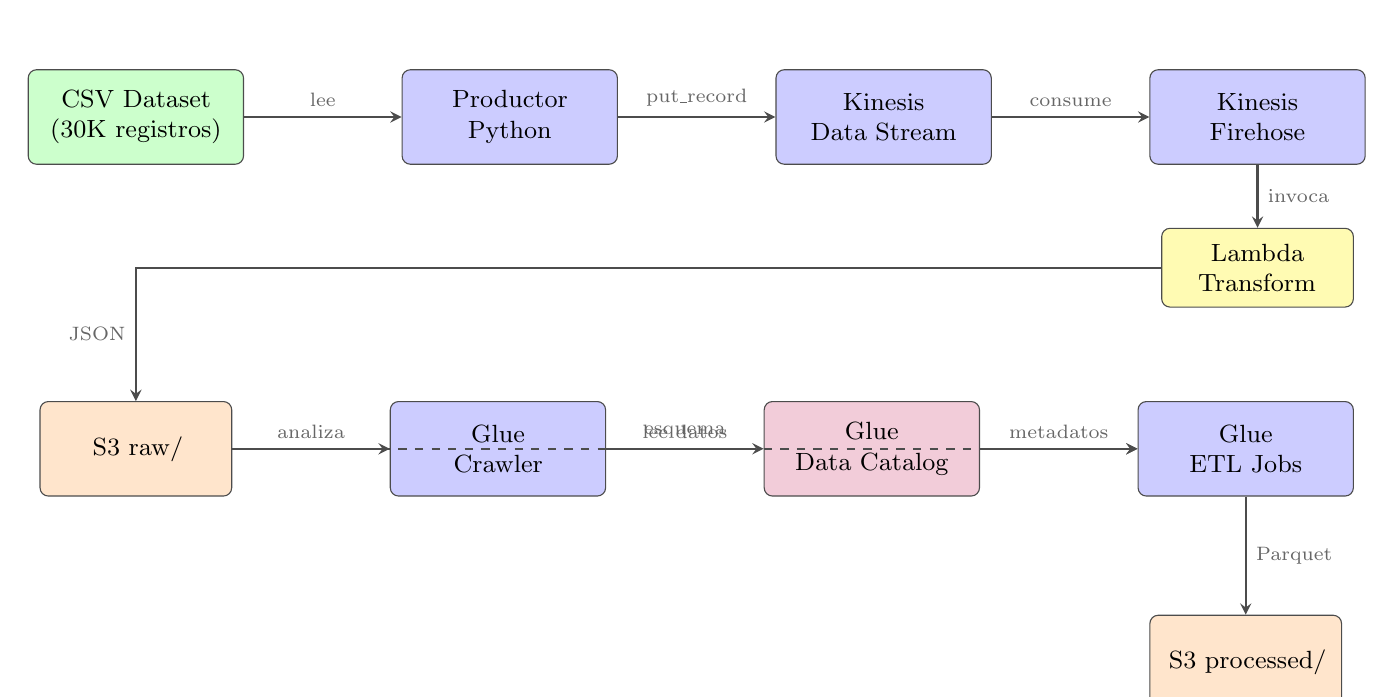
\begin{tikzpicture}[
    node distance=1.5cm and 2cm,
    % Estilos de nodos
    source/.style={rectangle, draw=black!70, fill=green!20, text width=2.5cm, text centered, minimum height=1.2cm, rounded corners=3pt, font=\small},
    process/.style={rectangle, draw=black!70, fill=blue!20, text width=2.5cm, text centered, minimum height=1.2cm, rounded corners=3pt, font=\small},
    storage/.style={rectangle, draw=black!70, fill=orange!20, text width=2.2cm, text centered, minimum height=1.2cm, rounded corners=3pt, font=\small},
    lambda/.style={rectangle, draw=black!70, fill=yellow!30, text width=2.2cm, text centered, minimum height=1cm, rounded corners=3pt, font=\small},
    catalog/.style={rectangle, draw=black!70, fill=purple!20, text width=2.5cm, text centered, minimum height=1.2cm, rounded corners=3pt, font=\small},
    arrow/.style={->, >=stealth, thick, black!70},
    label/.style={font=\scriptsize, text=black!60}
]

% Fila 1: Ingesta
\node[source] (csv) {CSV Dataset\\(30K registros)};
\node[process, right=of csv] (producer) {Productor\\Python};
\node[process, right=of producer] (kinesis) {Kinesis\\Data Stream};
\node[process, right=of kinesis] (firehose) {Kinesis\\Firehose};

% Lambda debajo de Firehose
\node[lambda, below=0.8cm of firehose] (lambda) {Lambda\\Transform};

% Fila 2: Almacenamiento y procesamiento
\node[storage, below=3cm of csv] (s3raw) {S3 raw/};
\node[process, right=of s3raw] (crawler) {Glue\\Crawler};
\node[catalog, right=of crawler] (catalog) {Glue\\Data Catalog};
\node[process, right=of catalog] (etl) {Glue\\ETL Jobs};

% S3 processed
\node[storage, below=1.5cm of etl] (s3proc) {S3 processed/};

% Flechas principales
\draw[arrow] (csv) -- (producer) node[midway, above, label] {lee};
\draw[arrow] (producer) -- (kinesis) node[midway, above, label] {put\_record};
\draw[arrow] (kinesis) -- (firehose) node[midway, above, label] {consume};
\draw[arrow] (firehose) -- (lambda) node[midway, right, label] {invoca};
\draw[arrow] (lambda) -| (s3raw) node[near end, left, label] {JSON};

\draw[arrow] (s3raw) -- (crawler) node[midway, above, label] {analiza};
\draw[arrow] (crawler) -- (catalog) node[midway, above, label] {esquema};
\draw[arrow] (catalog) -- (etl) node[midway, above, label] {metadatos};
\draw[arrow] (etl) -- (s3proc) node[midway, right, label] {Parquet};

% Conexión ETL lee de S3 raw
\draw[arrow, dashed] (s3raw) -- (etl) node[midway, above, label, sloped] {lee datos};

\end{tikzpicture}%
}
\caption{Arquitectura del Data Lake implementado con servicios AWS}
\label{fig:arquitectura}
\end{figure}

\vspace{0.5cm}
\noindent\textbf{Leyenda de colores:} 
\colorbox{green!20}{Verde} = Fuente de datos \quad
\colorbox{blue!20}{Azul} = Servicios AWS \quad
\colorbox{orange!20}{Naranja} = S3 \quad
\colorbox{yellow!30}{Amarillo} = Lambda \quad
\colorbox{purple!20}{Morado} = Catálogo

\subsection{Descripción del flujo}

\begin{enumerate}
    \item \textbf{Ingesta:} El productor Python lee el dataset CSV y envía 30,000 registros al Kinesis Data Stream.
    
    \item \textbf{Streaming:} Kinesis Data Stream recibe los registros y los mantiene disponibles para su consumo.
    
    \item \textbf{Transformación:} Kinesis Firehose consume los datos del stream, invoca la función Lambda para transformarlos y enriquecerlos.
    
    \item \textbf{Almacenamiento raw:} Los datos transformados se almacenan en S3 en formato JSON, particionados por año de lanzamiento.
    
    \item \textbf{Catalogación:} El crawler de Glue analiza los datos en S3 e infiere el esquema, creando una tabla en el Glue Data Catalog.
    
    \item \textbf{ETL:} Los jobs de Glue leen los datos del catálogo, aplican agregaciones y escriben los resultados en formato Parquet en la capa processed.
\end{enumerate}
\section{Presupuesto y estimación de costes}

A continuación se presenta una estimación de costes basada en el uso de los servicios AWS para esta práctica, considerando un escenario de uso real con 30,000 registros procesados diariamente.

\subsection{Supuestos de cálculo}

\begin{itemize}
    \item Región: US East (N. Virginia) - us-east-1
    \item Volumen de datos: 30,000 registros/día $\approx$ 15 MB/día
    \item Tamaño promedio por registro: 500 bytes
    \item Ejecución de jobs ETL: 1 vez al día
    \item Tiempo de ejecución de cada job: 5 minutos
\end{itemize}

\subsection{Desglose de costes}

\begin{table}[H]
\centering
\caption{Estimación de costes mensuales de AWS}
\begin{tabular}{lrrr}
\toprule
\textbf{Servicio} & \textbf{Unidad} & \textbf{Cantidad} & \textbf{Coste (\$/mes)} \\
\midrule
\multicolumn{4}{l}{\textit{Amazon S3}} \\
\quad Almacenamiento & GB & 0.5 & 0.01 \\
\quad PUT requests & 1000 req & 900 & 0.05 \\
\quad GET requests & 1000 req & 100 & 0.00 \\
\midrule
\multicolumn{4}{l}{\textit{Kinesis Data Streams}} \\
\quad Shard hour & horas & 720 & 10.80 \\
\quad PUT payload units & millones & 0.9 & 0.01 \\
\midrule
\multicolumn{4}{l}{\textit{Kinesis Data Firehose}} \\
\quad Data ingested & GB & 0.5 & 0.02 \\
\midrule
\multicolumn{4}{l}{\textit{AWS Lambda}} \\
\quad Requests & millones & 0.9 & 0.18 \\
\quad Duration (128MB) & GB-segundo & 100 & 0.00 \\
\midrule
\multicolumn{4}{l}{\textit{AWS Glue}} \\
\quad Crawler (DPU-hour) & horas & 0.5 & 0.22 \\
\quad ETL Jobs (G.1X) & DPU-hora & 5 & 2.20 \\
\quad Data Catalog & objetos & 10 & 0.00 \\
\midrule
\textbf{Total mensual} & & & \textbf{\$13.49} \\
\textbf{Total anual} & & & \textbf{\$161.88} \\
\bottomrule
\end{tabular}
\end{table}

\subsection{Notas sobre los cálculos}

\begin{itemize}
    \item \textbf{Kinesis Data Streams:} El coste principal proviene del shard-hour (\$0.015/hora). Con 1 shard activo 24/7, el coste mensual es de aproximadamente \$10.80.
    
    \item \textbf{AWS Glue:} Los jobs ETL se facturan por DPU-hora (\$0.44/DPU-hora). Con 2 workers G.1X ejecutándose 5 minutos diarios, el coste mensual es aproximadamente \$2.20.
    
    \item \textbf{Capa gratuita:} AWS ofrece capa gratuita para Lambda (1M solicitudes/mes) y S3 (5GB), lo que podría reducir los costes en un entorno de pruebas.
\end{itemize}

\section{Conclusiones}

\subsection{Conocimientos adquiridos}

Esta práctica ha permitido adquirir experiencia práctica en:

\begin{itemize}
    \item Diseño de arquitecturas de Data Lake siguiendo el patrón de capas (raw/processed).
    \item Implementación de pipelines de datos en tiempo real con Kinesis.
    \item Desarrollo de funciones Lambda para transformación de datos en streaming.
    \item Uso de AWS Glue para catalogación automática y procesamiento ETL con Spark.
    \item Configuración de servicios AWS mediante CLI, lo que facilita la automatización y reproducibilidad.
\end{itemize}

\subsection{Dificultades encontradas}

\begin{itemize}
    \item \textbf{Configuración de Firehose con particionamiento dinámico:} Requiere una configuración específica de la Lambda para devolver las claves de partición en el formato correcto.
    
    \item \textbf{Tiempos de espera:} Los servicios como Kinesis Stream y Firehose requieren tiempo para activarse, lo que debe considerarse en los scripts de automatización.
    
    \item \textbf{Depuración de jobs Glue:} La depuración de errores en Spark requiere revisar los logs de CloudWatch, lo que puede ser tedioso.
\end{itemize}

\subsection{Posibles mejoras}

\begin{itemize}
    \item Implementar Amazon Athena para consultas SQL directas sobre los datos en S3.
    \item Añadir Amazon QuickSight para visualización de dashboards.
    \item Configurar alertas de CloudWatch para monitorizar el pipeline.
    \item Implementar versionado del bucket S3 para recuperación ante errores.
    \item Usar AWS Step Functions para orquestar el flujo completo de forma más robusta.
\end{itemize}

\section{Demostraciones de Funcionalidad en AWS}

A continuación se presentan capturas de pantalla que demuestran el correcto funcionamiento de la arquitectura implementada.

Cabe destacar que, debido a que la practica la he realizado en su totalidad en la 
terminal con ".sh" y ".py", las imágenes corresponden a capturas de los resultados,
no al proceso de creación de la arquitectura. Para la creación de la misma, 
vaya a la sección \textit{Desarrollo de las actividades}.

\subsection{Amazon S3 - Data Lake}

\begin{figure}[H]
\centering
\includegraphics[width=0.9\textwidth]{Imagenes/0 Bucket.png}
\caption{Bucket S3 creado para el Data Lake}
\label{fig:bucket}
\end{figure}

\begin{figure}[H]
\centering
\includegraphics[width=0.9\textwidth]{Imagenes/1 datalake.png}
\caption{Estructura de carpetas del Data Lake en S3}
\label{fig:datalake}
\end{figure}

\begin{figure}[H]
\centering
\includegraphics[width=0.9\textwidth]{Imagenes/2 Datalake processed 1.png}
\caption{Datos procesados en la capa processed - Vista 1}
\label{fig:processed1}
\end{figure}

\begin{figure}[H]
\centering
\includegraphics[width=0.9\textwidth]{Imagenes/2 Datalake processed 2.png}
\caption{Datos procesados en la capa processed - Vista 2}
\label{fig:processed2}
\end{figure}

\subsection{AWS Glue - Catálogo de Datos}

\begin{figure}[H]
\centering
\includegraphics[width=0.9\textwidth]{Imagenes/3 databases.png}
\caption{Base de datos creada en AWS Glue Data Catalog}
\label{fig:databases}
\end{figure}

\begin{figure}[H]
\centering
\includegraphics[width=0.9\textwidth]{Imagenes/4 Tables.png}
\caption{Tablas detectadas por el Crawler en el catálogo}
\label{fig:tables}
\end{figure}

\begin{figure}[H]
\centering
\includegraphics[width=0.9\textwidth]{Imagenes/5 schema.png}
\caption{Esquema inferido automáticamente por el Crawler}
\label{fig:schema}
\end{figure}

\begin{figure}[H]
\centering
\includegraphics[width=0.9\textwidth]{Imagenes/6 Partitions.png}
\caption{Particiones detectadas por año de lanzamiento}
\label{fig:partitions}
\end{figure}

\begin{figure}[H]
\centering
\includegraphics[width=0.9\textwidth]{Imagenes/7 glue crawlers.png}
\caption{Crawler configurado y ejecutado correctamente}
\label{fig:crawlers}
\end{figure}

\subsection{Amazon Athena - Consultas}

\begin{figure}[H]
\centering
\includegraphics[width=0.9\textwidth]{Imagenes/8 queries 1.png}
\caption{Consulta SQL en Athena sobre los datos del Data Lake - Ejemplo 1}
\label{fig:queries1}
\end{figure}

\begin{figure}[H]
\centering
\includegraphics[width=0.9\textwidth]{Imagenes/8 queries 2.png}
\caption{Consulta SQL en Athena sobre los datos del Data Lake - Ejemplo 2}
\label{fig:queries2}
\end{figure}

\subsection{AWS Glue - Jobs ETL}

\begin{figure}[H]
\centering
\includegraphics[width=0.9\textwidth]{Imagenes/9 ETL.png}
\caption{Jobs ETL ejecutados correctamente en AWS Glue}
\label{fig:etl}
\end{figure}
\section{Anexos}

\subsection{Anexo A: Script completo de configuración (main.sh)}

\begin{lstlisting}[language=bash, caption={main.sh - Script completo de configuración}]
#!/bin/bash
# Script de configuracion del Data Lake para Steam Games

# --- CONFIGURACION INICIAL ---
export AWS_REGION="us-east-1"
export ACCOUNT_ID=$(aws sts get-caller-identity \
    --query Account --output text)
export BUCKET_NAME="datalake-steam-games-${ACCOUNT_ID}"
export ROLE_ARN=$(aws iam get-role --role-name LabRole \
    --query 'Role.Arn' --output text)

echo "Configuracion del Data Lake - Steam Games"
echo "Bucket: $BUCKET_NAME"
echo "Role ARN: $ROLE_ARN"

# 1. Crear bucket S3 y estructura
aws s3 mb s3://$BUCKET_NAME
aws s3api put-object --bucket $BUCKET_NAME --key raw/
aws s3api put-object --bucket $BUCKET_NAME --key raw/steam_games/
aws s3api put-object --bucket $BUCKET_NAME --key processed/
aws s3api put-object --bucket $BUCKET_NAME --key scripts/
aws s3api put-object --bucket $BUCKET_NAME --key errors/

# 2. Crear Kinesis Data Stream
aws kinesis create-stream \
    --stream-name steam-games-stream \
    --shard-count 1
aws kinesis wait stream-exists --stream-name steam-games-stream

# 3. Crear funcion Lambda
zip -j firehose.zip firehose.py
aws lambda create-function \
    --function-name steam-firehose-transform \
    --runtime python3.12 \
    --role $ROLE_ARN \
    --handler firehose.lambda_handler \
    --zip-file fileb://firehose.zip \
    --timeout 60 \
    --memory-size 128

export LAMBDA_ARN=$(aws lambda get-function \
    --function-name steam-firehose-transform \
    --query 'Configuration.FunctionArn' --output text)

# 4. Crear Firehose Delivery Stream
# (Ver codigo completo en seccion 2.3)

# 5. Configurar Glue
aws glue create-database \
    --database-input '{"Name":"steam_games_db"}'
aws glue create-crawler \
    --name steam-games-crawler \
    --role $ROLE_ARN \
    --database-name steam_games_db \
    --targets '{"S3Targets": [{"Path": "s3://'"$BUCKET_NAME"'/raw/steam_games/"}]}'

# 6. Subir scripts ETL
aws s3 cp energy_aggregation_daily.py \
    s3://$BUCKET_NAME/scripts/steam_aggregation_by_year.py
aws s3 cp energy_aggregation_monthly.py \
    s3://$BUCKET_NAME/scripts/steam_aggregation_by_genre.py

# 7. Crear jobs ETL
# (Ver codigo completo en seccion 2.4)

echo "Configuracion completada"
\end{lstlisting}

\subsection{Anexo B: Uso de Inteligencia Artificial}

Para el desarrollo de esta práctica se ha utilizado \textbf{GitHub Copilot} (modelo Claude) como asistente de programación. El uso de IA ha sido el siguiente:

\begin{itemize}
    \item \textbf{Generación de código:} Asistencia en la escritura de los scripts Python para el productor de datos y las funciones Lambda.
    \item \textbf{Comandos AWS CLI:} Ayuda en la sintaxis correcta de los comandos de AWS CLI para configurar los servicios.
    \item \textbf{Documentación:} Asistencia en la estructuración y redacción de este informe.
\end{itemize}

Todo el código generado ha sido revisado, probado y adaptado según las necesidades específicas del proyecto.

\section{Herramientas Utilizadas}
\subsection{Desarrollo}
Para el desarrollo de la práctica se han utilizado las siguientes herramientas:
\begin{itemize}
    \item \textbf{AWS CLI:} Herramienta de línea de comandos para interactuar con 
    los servicios de AWS, utilizada para automatizar la creación y configuración 
    de recursos.
    \item \textbf{Python 3.12:} Lenguaje de programación empleado para desarrollar 
    los scripts del productor de datos, funciones Lambda y jobs ETL en Glue.
    \item \textbf{Boto3:} SDK de AWS para Python, utilizado para interactuar 
    programáticamente con los servicios de AWS desde los scripts.
    \item \textbf{Visual Studio Code:} Entorno de desarrollo integrado (IDE) 
    utilizado para escribir y depurar el código Python, además de redactar la 
    documentación.
    \item \textbf{GitHub Copilot:} Asistente de programación basado en inteligencia 
    artificial que ha ayudado en la generación de código durante el desarrollo.
\end{itemize}
\subsection{Documentación}
Para la elaboración del informe y la documentación de la práctica se han 
utilizado las siguientes herramientas:
\begin{itemize}
    \item \textbf{LaTeX:} Sistema de preparación de documentos utilizado para 
    redactar el informe técnico de la práctica.
    \item \textbf{GitHub Copilot:} Asistente de inteligencia artificial que ha 
    colaborado en la redacción y estructuración del informe.
\end{itemize}
\subsection{Gestión de versiones}
Para el control de versiones y la gestión del código fuente se ha utilizado:
\begin{itemize}
    \item \textbf{Git:} Sistema de control de versiones distribuido utilizado para 
    gestionar los cambios en el código y la documentación.
    \item \textbf{GitHub:} Plataforma de alojamiento de repositorios Git, utilizada para 
    almacenar el código fuente y colaborar en el desarrollo.
\end{itemize}
\subsection{}
\section{Referencias y bibliografía}

\begin{itemize}
    \item Amazon Web Services. (2024). \textit{Amazon Kinesis Data Streams Developer Guide}. Recuperado de \url{https://docs.aws.amazon.com/streams/latest/dev/}
    
    \item Amazon Web Services. (2024). \textit{Amazon Kinesis Data Firehose Developer Guide}. Recuperado de \url{https://docs.aws.amazon.com/firehose/latest/dev/}
    
    \item Amazon Web Services. (2024). \textit{AWS Glue Developer Guide}. Recuperado de \url{https://docs.aws.amazon.com/glue/latest/dg/}
    
    \item Amazon Web Services. (2024). \textit{Amazon S3 User Guide}. Recuperado de \url{https://docs.aws.amazon.com/AmazonS3/latest/userguide/}
    
    \item Amazon Web Services. (2024). \textit{AWS Lambda Developer Guide}. Recuperado de \url{https://docs.aws.amazon.com/lambda/latest/dg/}
    
    \item Amazon Web Services. (2024). \textit{AWS Pricing Calculator}. Recuperado de \url{https://calculator.aws/}
\end{itemize}

\subsection{Código Fuente:}
El código fuente desarrollado para esta práctica está disponible en el siguiente 
repositorio de GitHub:
\begin{center}
\url{https://github.com/NicolasReyAlonso/Entrega_2_CN.git}
\end{center}

\end{document}
